\documentclass[11pt]{article}
\usepackage{graphicx}
\usepackage{array}
\usepackage{xcolor}
\usepackage[a4paper,total={8in,10in}]{geometry}
\usepackage{mdframed}
\usepackage{geometry}
\usepackage{hyperref}
\begin{document}
\begin{mdframed}[backgroundcolor=orange]
~
\begin{center}
\begin{Huge}
\color{white}{\fontfamily{pbk}\selectfont SIDDHANT}\color{gray}{\fontfamily{pbk}\selectfont\textbf{ BHAMBRI}}
\end{Huge}
\end{center}
\begin{center}
\begin{large}
\color{white}\emph{Aiming to use technology to bring a considerable positive change for mankind}
\end{large}
\end{center}
\end{mdframed}
\begin{minipage}{1.00\linewidth}
\begin{center}
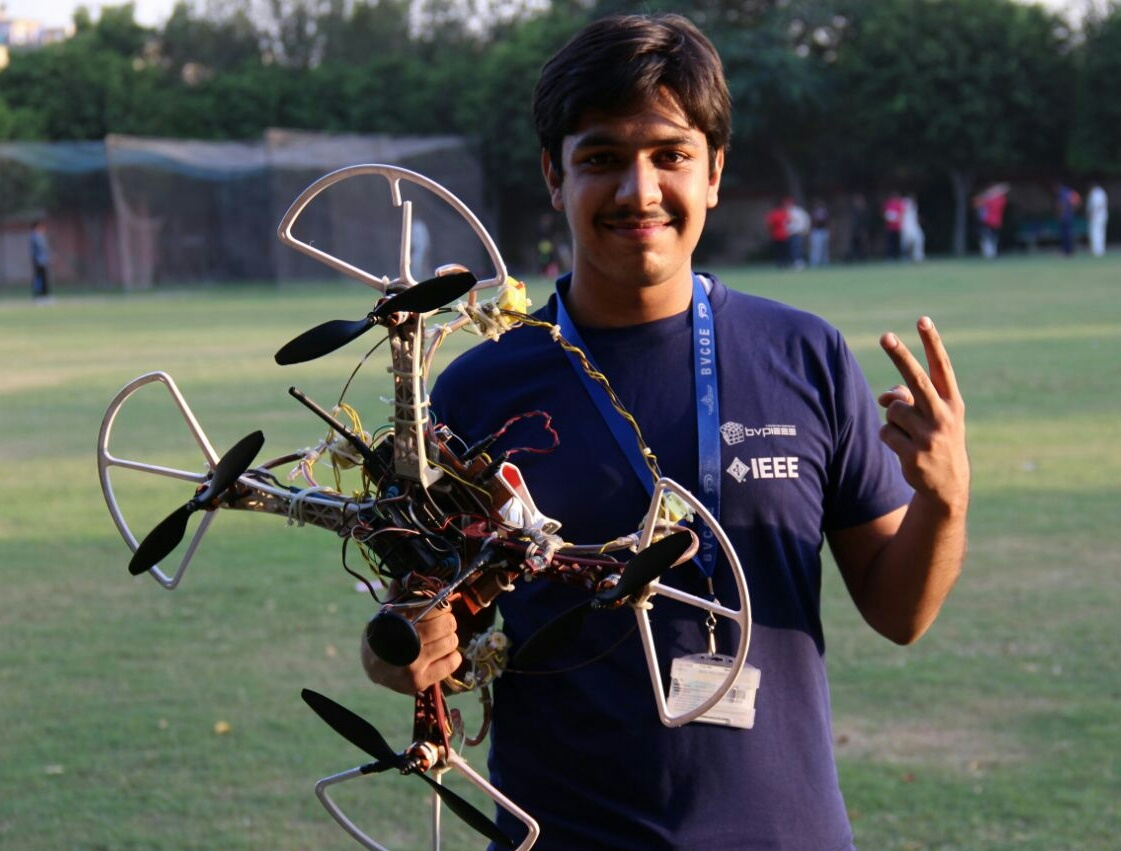
\includegraphics[scale=0.185]{siddhant_image}
\end{center}
\end{minipage}
\begin{flushleft}
	\section{\color{green}Per\color{purple}s\color{black}onal D\color{purple}e\color{black}tai\color{purple}l\color{black}s}
	~
\textbf{Address-}    
    886/2A 
    Preet Vihar, Rohtak.\\
    ~
    Haryana\\
    ~
    124001\\
    ~
    \textbf{Contact}-
    +91 9728466229\\
~
\textbf{E-mail-} \href{mailto:siddhantbhambri@gmail.com}{siddhantbhambri@gmail.com}\\
 ~   
    \textbf{LinkedIn-}
    \href{http://www.linkedin.com/in/siddhant-bhambri-27b7a5111}{http://www.linkedin.com/in/siddhant-bhambri-27b7a5111}
\end{flushleft}

\section{\color{yellow}Edu\color{black}cational Qualifications}
\begin{center}
\begin{tabular}{ |m{4cm}| m{4cm}| m{2cm}| m{3cm}| }
\hline
&&&\\
\begin{center}
\textbf{{ Course/Examination }}
\end{center}&\begin{center}\textbf{ Institute/University }\end{center}&\begin{center}\textbf{ Year of passing }\end{center}&\begin{center}\textbf{ Performance }\end{center}\\
\hline
&&&\\
\begin{center}
B.Tech, Electronics and Communication Engineering
\end{center}& \begin{center}
Bharati Vidyapeeth's College Of Engineering
\end{center}&\begin{center}
2019
\end{center}& \begin{center}
71.00 (C) (up to third semester)
\end{center}\\
\hline
\begin{center}
CBSC (SCIENCE-PCM)\\
XIIth
\end{center}&
\begin{center}
(CBSE) Model School Rohtak, Haryana
\end{center}&
\begin{center}
2015
\end{center}&
\begin{center}
77.00 percent(agg)
\end{center}\\
\hline
\begin{center}
CBSE\\
Xth
\end{center}&
\begin{center}
(CBSE) Model School Rohtak, Haryana
\end{center}&
\begin{center}
2013
\end{center}&
\begin{center}
8.8 CGPA
\end{center}\\
\hline
\end{tabular}
\end{center}

\end{document}